\subsection{Resultater}
Resultater inddeles i en grænseflade og dertilhørende controller, som det fremgår af \autoref{fig:MVCresultater}. 

\begin{figure} [H]
\centering
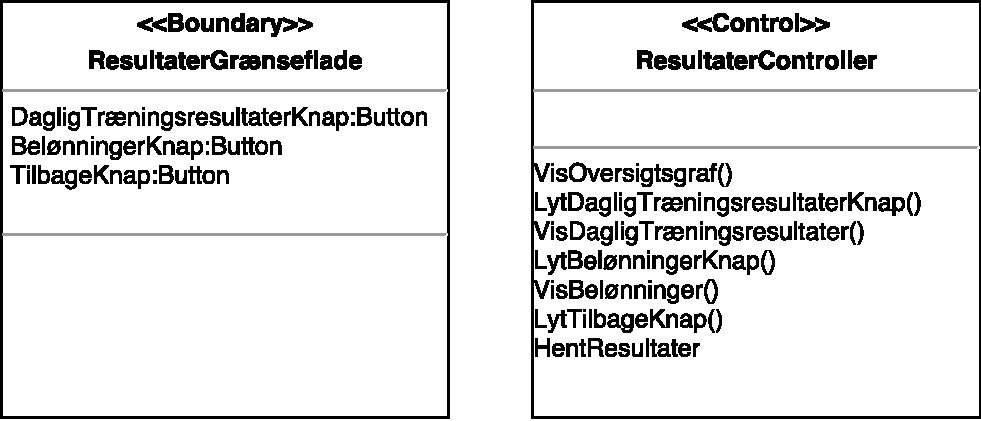
\includegraphics[width=0.9\textwidth]{figures/MVC/Resultater}
\caption{Designklasser for resultater}
\label{fig:MVCresultater}
\end{figure}

\noindent
I \textit{ResultaterGrænseflade} er der opstillet knapper af typen button for daglig træningsresultater belønninger og en tilbage. Disse indikerer ved tryk, at brugerens har valgt en af de mulige handlinger. 
 
Der er til \textit{ResultaterGrænseflade} opstillet en \textit{ResultatController}, der har til formål at hente nye resultater fra dagens træning i træningscontrolleren, når resultater tilgås via hovedmenugrænsefladen. Herefter vises en oversigtsgraf over udført træning. Træningscontrolleren fremgår af \autoref{fig:MVCTraening}.
Controlleren lytter på om brugeren trykker på de angivne knapper i grænsefladen for resultater og viser valgt handling, hvis dette er tilfældet. 
